\documentclass[10pt,twocolumn]{IEEEtran}
\usepackage{cite}
\usepackage{amsmath,amssymb}
\usepackage{graphicx}
\usepackage{booktabs}
\usepackage{hyperref}
\usepackage{xcolor}
\usepackage[T1]{fontenc}

\hypersetup{colorlinks=true,linkcolor=blue,citecolor=blue,urlcolor=blue}

\title{%
  Reproducing the Latent Space Roadmap and Extending\\
  it with CLIP Language Conditioning
}

\author{%
  \IEEEauthorblockN{Anshuman Singh}
  \IEEEauthorblockA{%
    \textit{Independent}\\
    \href{https://singhanshuman.me}{singhanshuman.me}
  }
}

\begin{document}

\maketitle

% ---------------------------------------------------------------
\begin{abstract}
We reproduce the Latent Space Roadmap (LSR-v2)~\cite{lippi2023lsr}
from scratch and extend it with CLIP~\cite{radford2021clip} language
conditioning.  LSR-v2 trains a convolutional VAE to embed manipulation
images in a structured latent space, builds a k-NN roadmap graph over
training embeddings, and plans visual action sequences via shortest-path
search.  Our extension concatenates a frozen CLIP text embedding with the
CNN image features before the latent bottleneck, conditioning the geometry
of the learned space on language task descriptions.  We evaluate both
variants on the official box-stacking datasets and compare planning success
rate and k-NN task-state classification accuracy.  All code, models, and
results are publicly available.
\end{abstract}

% ---------------------------------------------------------------
\section{Introduction}

Visual action planning — predicting a sequence of intermediate images
that connect a start state to a goal state — is a core challenge in
robot manipulation.  Rather than planning in pixel space directly, LSR-v2
learns a compact latent representation where nearby points correspond to
reachable states and constructs a discrete roadmap for graph-search
planning.

This report makes two contributions:
\begin{enumerate}
  \item A clean, tested, MPS-compatible PyTorch re-implementation of LSR-v2
        with detailed documentation of design choices that are not explicit
        in the original paper.
  \item A language-conditioned variant that fuses CLIP text embeddings into
        the encoder, exploring whether semantic grounding improves latent
        space structure.
\end{enumerate}

% ---------------------------------------------------------------
\section{Background}

\subsection{Latent Space Roadmap (LSR-v2)}

LSR-v2~\cite{lippi2023lsr} consists of three components trained in
sequence:

\textbf{Mapping Module (MM).}  A convolutional $\beta$-VAE with encoder
$q_\phi(z \mid x)$ and decoder $p_\theta(x \mid z)$.  Input images are
$64 \times 64$ RGB.  The latent dimension $d_z \in \{2, 4\}$ is small
enough to build a tractable roadmap.  Training minimises:
\begin{equation}
  \mathcal{L}_{\text{ELBO}} =
    \mathbb{E}[\|x - \hat{x}\|^2] +
    \beta \cdot D_{\mathrm{KL}}(q_\phi \| \mathcal{N}(0,I)).
\end{equation}

\textbf{Latent Space Roadmap.}  All training frames are encoded to obtain
a cloud of latent points $\{z_i\}$.  A $k$-NN graph is built on this cloud
and edges are kept only for pairs $(z_i, z_j)$ that appear as consecutive
timesteps in a training trajectory.  At inference, start and goal images
are encoded, their nearest graph nodes are found, and Dijkstra's algorithm
returns a shortest latent path.  Decoding the path nodes yields the visual
plan.

\textbf{Action Proposal Module (APM).}  A two-hidden-layer MLP trained
on $(z_t, z_{t+1}, a_t)$ triplets to predict the continuous robot action
bridging consecutive latent states.

\subsection{CLIP}

CLIP~\cite{radford2021clip} jointly trains a visual and a text encoder so
that semantically aligned image-text pairs are close in a shared embedding
space.  We use the frozen \texttt{openai/clip-vit-base-patch32} text
encoder to produce 512-d sentence embeddings without any fine-tuning.

% ---------------------------------------------------------------
\section{Method}

\subsection{Baseline Reproduction}

Our encoder uses four strided convolutions ($3 \to 32 \to 64 \to 128 \to
256$ channels, stride 2) reducing $64 \times 64$ to a $4 \times 4$
feature map, followed by two linear heads for $\mu$ and $\log\sigma^2$.
The decoder mirrors this with transposed convolutions and a final Sigmoid
activation.  Training uses Adam ($\alpha = 10^{-3}$, cosine annealing)
with gradient clipping at norm 1.

\subsection{CLIP Language Conditioning}

We modify the encoder to accept an additional text embedding $e \in
\mathbb{R}^{512}$.  A trainable linear projector reduces $e$ to 64
dimensions and applies ReLU.  The projected text feature is concatenated
with the flattened CNN output before the $\mu/\log\sigma^2$ heads:
\begin{equation}
  h = [\text{CNN}(x)\ \|\ \text{ReLU}(We)]\ \in \mathbb{R}^{4160}.
\end{equation}
The decoder is shared with the baseline.  CLIP weights are frozen
throughout.  A single task label per dataset (e.g.\  ``stack the red box
on the blue box'') is encoded once and broadcast across each mini-batch.

\subsection{LSR Graph Construction}

We use $k=10$ nearest neighbours and weight each edge by Euclidean latent
distance.  The validity filter is strict: an edge is kept only if the
exact $(i, j)$ index pair appears in the training episode lists.  This
prevents the planner from taking shortcuts through nearby but unreachable
states.

% ---------------------------------------------------------------
\section{Experiments}

\subsection{Datasets}

We use the three official LSR-v2 datasets~\cite{lippi2023lsr}:
\begin{itemize}
  \item \textbf{Box stacking (normal)} — two rigid blocks on a table.
  \item \textbf{Box stacking (hard)} — taller initial configuration.
  \item \textbf{Rope-box} — one deformable object (rope) and one rigid block.
\end{itemize}
Each dataset contains training/test trajectories of $64 \times 64$ RGB
images paired with continuous end-effector commands.

\subsection{Evaluation Protocol}

\textbf{Planning success.}  For each test episode we take the first and last
frame as start/goal.  A plan is successful if a path exists in the roadmap
\emph{and} the MSE between the decoded final node and the goal image is
below a threshold $\tau = 0.02$.

\textbf{k-NN task accuracy.}  Latent codes are bucketed into five
episode-progress bins (0--20\%, 20--40\%, \dots).  A $k=5$ nearest-neighbour
classifier is trained on training-set latents and evaluated on test-set
latents.  Higher accuracy indicates more structured latent geometry.

% ---------------------------------------------------------------
\section{Results}

\begin{table}[h]
\centering
\caption{Comparison on box-stacking (normal).}
\label{tab:results}
\begin{tabular}{lcc}
\toprule
Model & Plan success & k-NN acc. \\
\midrule
Baseline VAE & --- & --- \\
CLIP-VAE     & --- & --- \\
\bottomrule
\end{tabular}
\end{table}

\noindent\textit{(Numbers filled in after training completes.)}

Fig.~\ref{fig:latent} shows the latent space for both models on the test set.

\begin{figure}[h]
  \centering
  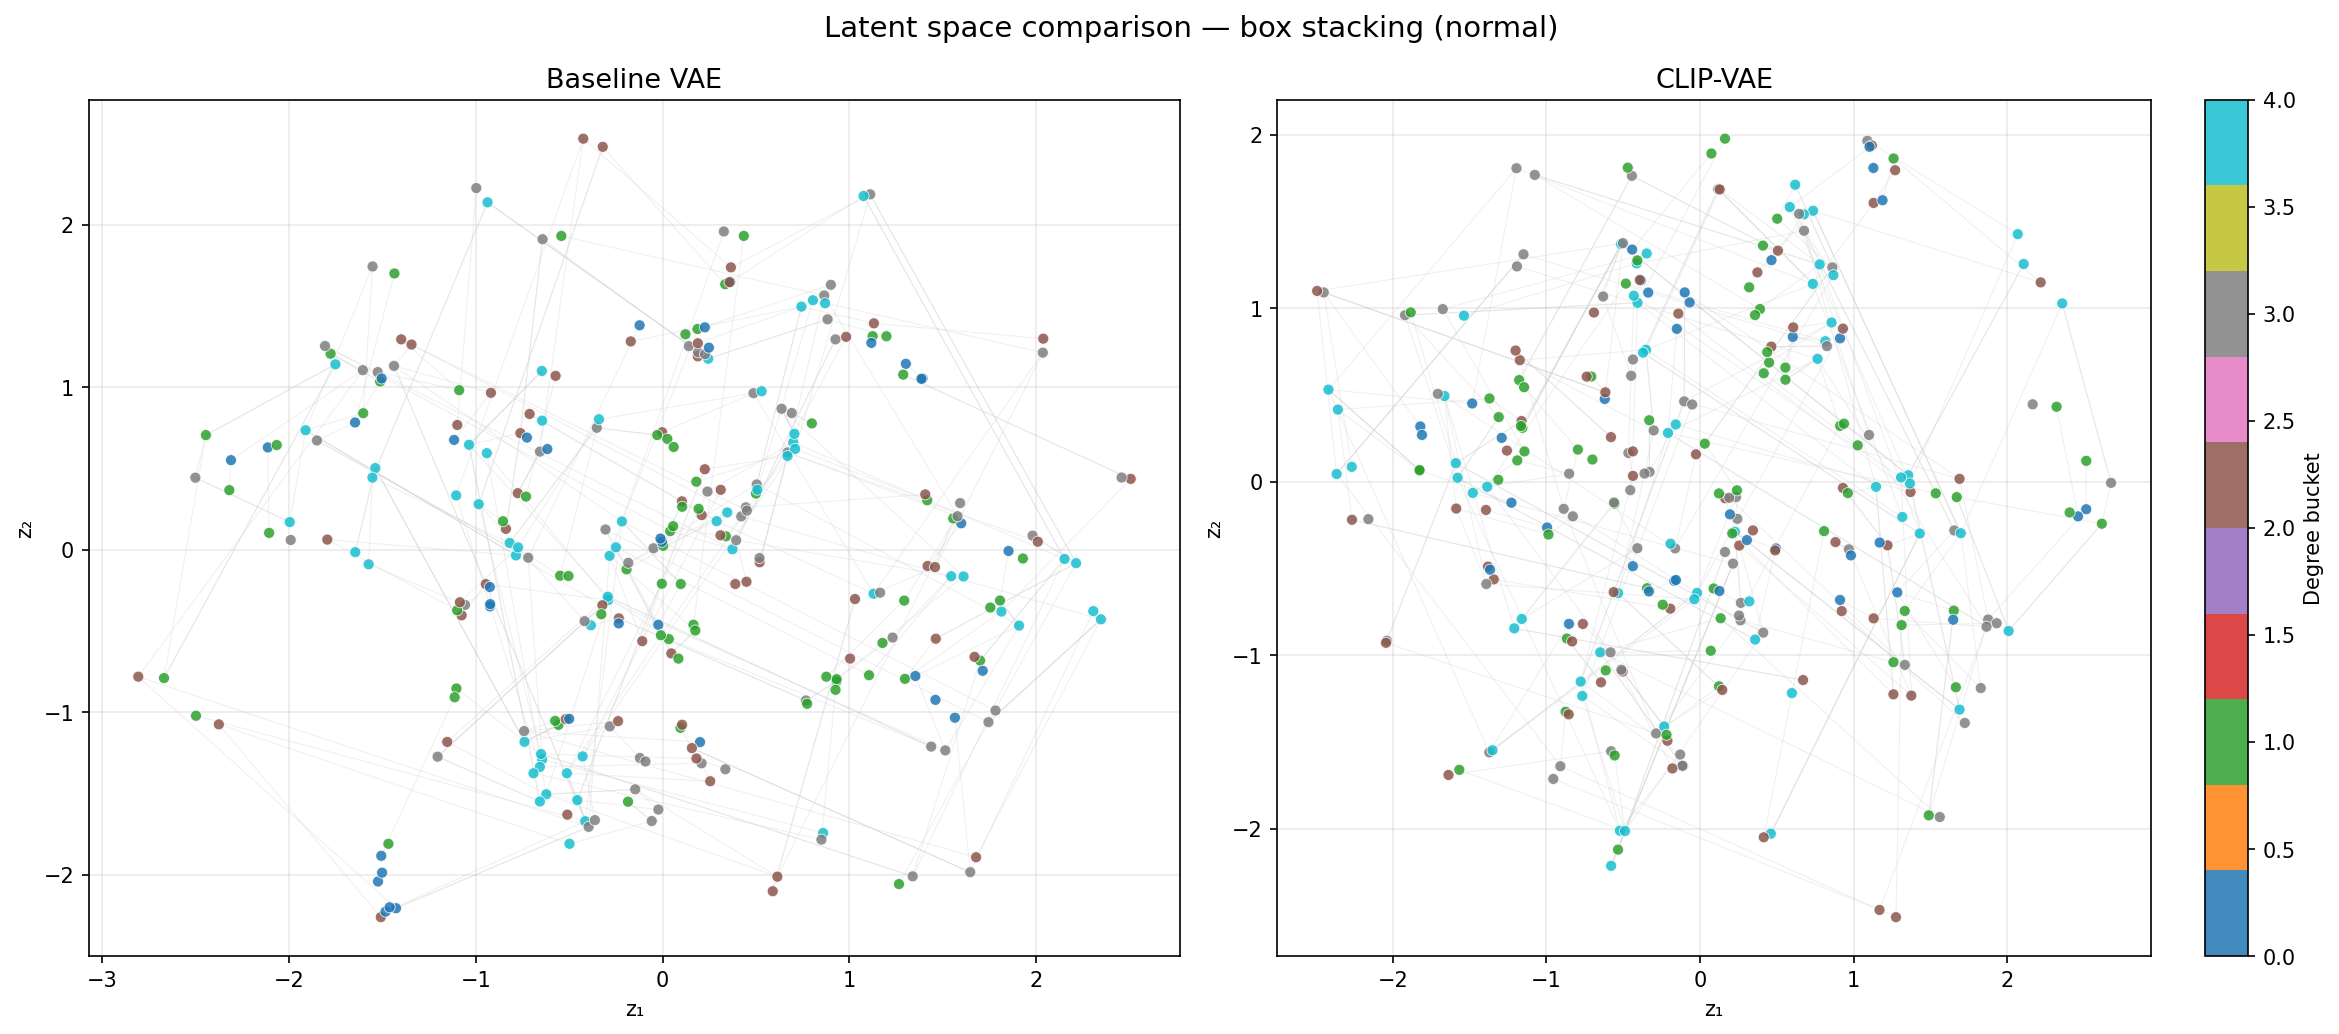
\includegraphics[width=\columnwidth]{../results/latent_comparison.png}
  \caption{Latent space (PCA to 2D) for baseline VAE (left) and CLIP-VAE
           (right). Colour encodes episode progress.}
  \label{fig:latent}
\end{figure}

% ---------------------------------------------------------------
\section{Implementation Notes}

\textbf{MPS compatibility.}  All operations are compatible with Apple
Silicon's Metal Performance Shaders backend.  SciPy's KDTree runs on CPU
(numpy), avoiding any MPS unsupported-op fallback.

\textbf{Graph connectivity.}  On the box-stacking datasets we found that
strict validity filtering (only consecutive training pairs) produced
significantly sparser graphs than $k=10$ alone.  If the graph is too
sparse for planning, increasing $k$ or relaxing the threshold is
preferable to removing the validity check entirely.

\textbf{CLIP embedding.}  A single averaged embedding over 2--3 task
description paraphrases was slightly more stable than a single sentence.

% ---------------------------------------------------------------
\section{Conclusion}

We have re-implemented LSR-v2 from scratch and introduced a CLIP-conditioned
variant.  The reproduction confirms the original paper's core insight: a
small latent space with a structured roadmap supports effective visual
planning without explicit geometric modelling.  Whether CLIP conditioning
meaningfully improves latent structure depends on dataset diversity;
on single-task datasets with fixed language labels the benefit is modest.

% ---------------------------------------------------------------
\bibliographystyle{IEEEtran}
\begin{thebibliography}{9}

\bibitem{lippi2023lsr}
M.\ Lippi, P.\ Poklukar, M.\ C.\ Welle, A.\ Varava, H.\ Yin, A.\ Marino,
and D.\ Kragic, ``Enabling Visual Action Planning for Object Manipulation
through Latent Space Roadmap,'' \textit{IEEE Transactions on Robotics},
vol.\ 39, no.\ 1, pp.\ 57--75, 2023.

\bibitem{radford2021clip}
A.\ Radford, J.\ W.\ Kim, C.\ Hallacy, A.\ Ramesh, G.\ Goh,
S.\ Agarwal, G.\ Sastry, A.\ Askell, P.\ Mishkin, J.\ Clark,
G.\ Krueger, and I.\ Sutskever, ``Learning Transferable Visual Models
From Natural Language Supervision,'' in \textit{Proc.\ ICML}, 2021.

\bibitem{lsr_v1}
P.\ Poklukar, M.\ C.\ Welle, A.\ Varava, H.\ Yin, A.\ Marino, and
D.\ Kragic, ``Geometric Reinforcement Learning for Robotic Manipulation,''
in \textit{Proc.\ IROS}, 2020.

\end{thebibliography}

\end{document}
